%%%%%%%%%%%%%%%%%%%%%%%%%%%%%%%%%
% 6CCS3PRJ Final Year Individual Project Report
% luke.day@kcl.ac.uk
%%%%%%%%%%%%%%%%%%%%%%%%%%%%%%%%%
\documentclass[11pt]{informatics-report}
\usepackage{soul, xcolor}
\usepackage{amssymb}
\usepackage{amsthm}
\usepackage{natbib} % References
\usepackage{minted} % Code listings
\usepackage[linesnumbered, ruled,noline]{algorithm2e}
\usepackage{tabularx}
\usepackage{mathtools}
\DeclarePairedDelimiter\abs{\lvert}{\rvert}
\usemintedstyle{vim}

%%%%%%%%%%%%%%%%%%%%%%%%%%%%%%%%%
% Front Matter - project title, name, supervisor name and date
%%%%%%%%%%%%%%%%%%%%%%%%%%%%%%%%%
\title{Code Contribution Assessment}
\author{Fahim Mohammed}
\studentID{1681338}
\supervisor{Jeroen Keppens}

\date{\today}

\abstractFile{FrontMatter/abstract.tex}
\ackFile{FrontMatter/acknowledgements.tex} %Remove line if you do not want acknowledgements

\begin{document}
\createFrontMatter
\onehalfspacing
\tableofcontents
\doublespacing

%%%%%%%%%%%%%%%%%%%%%%%%%%%%%%%%%
% Report Content
%%%%%%%%%%%%%%%%%%%%%%%%%%%%%%%%%
% You can write each chapter directly here or in a separate .tex file and use the include command.

\chapter{Introduction}
The process this project sets out to analyse is known as code contributions, which help identify an author for a piece of code within a codebase and rating the individual based on the volume of said contribution in respect to the contributions of the other authors in the repository \citep{10.1007/s10664-017-9575-4}. The problem we set out to solve is relevant to student group projects where the current systems and metrics used only display a rudimentary idea of code contribution. Using this approach to code attribution can also further be applied to crowdsourced software since the public or a large community are allowed to contribute to a piece of software.

It seems that knowing what percentage of code has been generated by a particular user is a multidisciplinary interest; academic interest \citep{kilgour_gray_sallis_macdonell_2012} is obvious given the fact that most academic projects require multiple contributors. There is also a clear interest from software engineers \citep{linares-vasquez_hossen_dang_kagdi_gethers_poshyvanyk_2012} but it holds potential applications for revenue attribution to internal and open-source contributors. When it comes to student group projects, the assessor will be able attribute marks more accurately. However, the current solutions are very limited for measuring code contributions, with some approaches having limitations in accurately measuring the size of contributions \citep{git-author_2013}.

\section{Aims and Challenges}
There are numerous numbers of difficulties when measuring code contributions in a student group project when compared to a project with a single developer:
\begin{itemize}
    \item \textbf{Project Size}: Repository of code can span over multiple files and any user on the team can freely edit them. 
    \item \textbf{Code Variability}: Repository can involve a range of programming languages and different frameworks for development.
    \item \textbf{Revision Control}: Code is constantly being revised and committed by different users and the revision control software being used dictates the accuracy of the existing systems.
    \item \textbf{Ranking Metrics}: No agreed approach to metrics with existing measures not differentiating on the quality of contributions.
    \item \textbf{Perspectives}: Different individuals will have a different perspective on what is seen as an ideal ranking system.
\end{itemize}

These challenges present the problem which has yet to be applied to academic marking in group projects. This project proposes a ranking algorithm that measures code contributions by incorporate measurements on quantity of code contributed by each user and measurements of code quality. The proposed solution from this project has the following properties:
\begin{itemize}
    \item \textbf{Language agnostic}: The algorithm can be applied to files containing any form of text from C++ code to HTML or Python. 
    \item \textbf{Independent of Size}: The size of the project does not matter whether it is over large files or over a plethora of files.
    \item \textbf{Awareness of code quality}: The algorithm quantifies the quality of contributions through the number of commits it persists through from creation.
    \item \textbf{Versatility to change}: The algorithm uses diffs like Git to track any code changes such as insertions, deletions or replacements of code. It is also able to track the movement or rearrangement of code.

\end{itemize}

\section{Report Structure}
This report will start with a short overview into the background of relevant topics, followed by a literature review of some of the relevant ranking algorithms in use for the purpose of identifying code contributions. This will be followed by the requirements set out for this project, the specification for the algorithm, and the final design of the ranking algorithm.

Then, the report will step through the process of implementation for the proposed ranking algorithm chronologically. The chapter introducing the implementation will also address any challenges encountered during development and the solutions which were created as a result. 

Following this, the report will contain a short insight into the professional concerns which could be raised when the project is applied to the student group project repositories. This will be followed by a collection of case studies that will test the algorithm on certain test cases and also multiple real student group projects of different sizes, where the results of these tests will be compared and discussed. 

Next, the outcomes of the developed software and testing will be evaluated, with the strengths and weaknesses of the whole project will be identified. Conclusively, a summary of what has been learnt throughout the project and how the project could possibly be continued in the future will be contained in the conclusion chapter.
\chapter{Background}
This chapter will explore current and existing applications of estimating code contributions and will include a literature review of various measures in use currently.
\section{Definitions}
Code contribution concerns identifying which user in the repository was the author of a section of the codebase and ranking the aforementioned user based on the relative extent of the contribution when compared to other authors in the repository \citep{10.1007/s10664-017-9575-4}.

This project will also be looking at and measuring code quality which in this project will be defined as the number of commits it persists through from creation (i.e. if the code is older, it is more likely to be important, giving it a reason to be in the codebase) \citep{10.1093/iwc/iwx010}. A codebase is a collection of source code that is used to create and build a piece of software \citep{wiki:codebase}. In relation to the project, codebases are the subset of the repositories in which the student group projects are stored. Here, a repository is a data structure that is used in version control (through version control software such as Git and Subversion) to store metadata about a set of files or directory structure \cite{collins-sussman_fitzpatrick_pilato_2004}.

\section{Literature Review}
Existing ranking methods that have been explored seem to utilise features and properties provided as a part of existing version control systems. These methods seek to calculate how much code is implemented by each user to the target project by measuring the contributions to the files in the project. However, this only looks into one of the levels of abstraction available for analysis when trying to measure code contributions.

The top level of abstraction available for analysis is to relate the contributions for one user and comparing that the total contributions to a repository. This is one of the approaches currently in use by the marking system for the student group projects. This approach uses the basis of which version control systems work, in which a user contributes a collection of work for completing a single task (known as a commit). Trying to formalise this approach, if \textit{c} is defined as the total number of commits made to an entire repository and \textit{$c_u$} is the total number of commits made by a user \textit{u}, then the relative proportion of the contribution by the user \textit{u} would be: 
\begin{equation} \label{eq:1}
  contribution_u = \frac{c_u}{c}
\end{equation}

However, by definition, a commit can contain multiple changes to multiple files, making the method explained in the equation \ref{eq:1} above inaccurate. Another approach uses the number of files affected and changed by each commit \citep{10.1145/2025113.2025119}. In this approach, the concept known as "touching" is shown in the following equation:
\begin{equation} \label{eq:2}
    touch_u = \frac{x_u}{x}
\end{equation}
where \textit{x} is the total number of changes in the repository throughout all the files and \textit{$x_u$} denotes all the changes made by the user \textit{u}. These approaches work when a high level view of contributions are required. 

Another level of abstraction is to look at contributions on a modular level. Here, modules refer to high level components that can be found in files such as functions and classes \cite{10.1145/2601248.2601283}. The formula for this concept is the same to equation \ref{eq:1} and \ref{eq:2} with the formula being applied to modules instead of considering commits.

A lower level of abstraction can identify the line changes made to the files by using algorithms applied by version control systems to track file changes. These algorithms are based on the \textit{longest common subsequence} problem \citep{10.1145/322063.322075} and the many implementations of these algorithms are known as \textit{diff}. For instance, the diff algorithm used by the git version control system can track line-level changes in a repository. These line changes could be line additions, deletions, or modifications. Awarding of these additions and modifications goes to the user that contributed a particular commit. This ranking system is currently used by tools such as \textit{git-fame} \citep{oleander_2020} and \textit{git-blame} \citep{git-blame_2020}. However, these tools are limited because modifications are always attributed to last person to modify it, meaning some users may have commits where their lines of code were removed or replaced. 

Following this drawback, an improved version of these tools was devised called \textit{git-author} which is able to "recover more information than git-blame for about 10\% of lines" \citep{git-author_2013}. This method uses a graph of line changes and produces a weighted score for each user and each line. It is also able to detect line movement using a diff tool which has been adapted called \textit{ldiff} \citep{5070564}. To produce a weighted score, the \textit{ldiff} tool utilises the Wagner-Fischer algorithm \citep{10.1145/321796.321811} through a set of line comparisons. Looking into the algorithm, the method described is partially used as a character-level measure.

A different perspective to producing rankings for contributions is to calculate the amount of time spent working on a repository for a project. This can be measured if the time a user starts working on the project is recorded, \textit{$T_{i,start}$}, and the time the user stops working on the project, \textit{$T_{i,end}$}, where \textit{i} is the session number from \textit{n} sessions. So, the time spent during a session on the project can be given by:
\begin{equation}
    T_i = T_{i,end} - T_{i,start} 
\end{equation}

As a result, the total time spent on the project by all contributors is \textit{$T = \sum^{N}_{i=1} T_i$}. However, this measure is difficult to measure in a group project in a mostly online environment since the start time for each session may be unavailable because of system restrictions. For example, \textit{git} makes the commit time available which can be used as the end time for a session, but the start time for a session is not available because most users using \textit{git} do not record when they start working on a file. However, the commit time can be used to find the time difference between two commits which can be expressed as the following:
\begin{equation} \label{eq:3}
    \delta T_{i, i-1} = T_{i,end} - T_{i-1,end} = B_{i,i-1} + T_i
\end{equation}
where {$B_{i,i-1}$} denotes the time spent where the user is not working on the project and is between sessions \textit{i} and \textit{i-1}. If \textit{B} is small enough, the first part of \ref{eq:3} gives a good approximation of the time spent on each session $T_i$. On the other hand, if B is too large (i.e. sleeping) then the previous deduction is proved obsolete. 

Some studies have used code contribution algorithms to predict bugs and the quality of the end product produced by a project \citep{FOUCAULT2015102}. The aforementioned studies have discussed this with regards to whether having many users working on a piece of code is effective in limiting bugs (known as extreme programming) \citep{796139} or if having a single senior author who authored most of the code is more effective \citep{10.1145/2025113.2025119}. 

All the algorithms discussed in this section have both similarities and limitations. All the algorithms are language and size independent but are not resistant to change, are not aware of code quality, and are unable to track movements and rearrangements of code. The only exception to this is \textit{git-author} which is able to track the movements and rearrangements. However, none of the algorithms are able to recognise the code quality of commits from users and all of them favour contributors that have multiple commits. Namely, these algorithms look at the volume of code contributions (at different levels of abstraction) and do not look into code quality.

\chapter{Specifications}
 The application is intended for users that are completing group projects as part of their $2^{nd}$ year software engineering module (5CCS2SEG) to visualise their relative contribution to their group. This chapter will define the various requirements which are needed for this project's accompanying software, from functional requirements to hardware requirements.

\section{Brief}
The main goal of this project is to create a means of reporting code contributions to a shared code repository using an algorithm to extract the data from repository. The application must display the result of the algorithm in a meaningful way, whether that be a visualisation of graphs or a set of metrics.

\section{Requirements}
The requirements for this project have been displayed in a tabular form with each requirement being accompanied with the relevant specification for the application being developed. These requirements were developed after studying the existing algorithms that were mentioned in last chapter. Below are the requirements that will need to accomplished by the software being produced:  
\\

\begin{tabularx}{1\textwidth}{
  | >{\raggedright\arraybackslash}X 
  | >{\centering\arraybackslash}X 
  | >{\raggedleft\arraybackslash}X | }
\hline
\textbf{Requirement} & \textbf{Specification} \\ \hline

The user must be able to access the application using their GitHub credentials. & Implement an OAuth integration to the application to allow users to login to the application using their GitHub accounts. \\ \hline

The user must be able to visualise their contributions in a selected repository. & Create basic and user-friendly visualisations that are produced after the repository has been analysed. \\ \hline

The user must receive accurate and correct code contribution information from the application. & Create an algorithm for analysing code contribution using existing pattern matching algorithms. \\ \hline

The user should be able to navigate the web application without guidance. & Create a simple, user-friendly user interface and make the application as accessible as possible. \\ \hline

The user should be able to allow contribution analysis for all their repositories (both private and public). & Implement a dynamic Model-View-Controller infrastructure that creates views and analyses repositories depending on the user's chosen repository. \\ \hline

The user should be able to visualise the contributions of all contributors in a repository. & Create a separate view that displays all users' contribution visualisations, instead of being compared to one user (user vs rest of team). \\ \hline 

The user could be able to see the algorithm's attribution for each user in each file of a repository. & Create a view that displays each file after the contributions have been attributed to the contributors of a repository. This would require the controller for said view to dynamically highlight each user's character changes in a file. \\ \hline

\end{tabularx}
\chapter{Design}
The algorithm that has produced as a part of this project has two main components: the first component calculates and finds blocks of code which match between two revisions of the code (i.e. between two commits), the second uses the matching blocks to calculate the code contributions for all of the users that contributed to a single file. The proposed algorithm's abstraction analyses the repository at the character level and has the properties discussed in Section 1.1, namely, awareness of code quality, and versatility to change. The way the project was approached was inspired by a study carried out to test and compare quality of open-source contributions on Wikipedia \citep{10.1145/1531674.1531682}. While this research project was looking into a single language of English and using a tokenisation approach, this project aims to be independent of programming languages. This property is more useful in a student group project environment. The approach proposed for this project (using character-level abstraction) has two main reasons and advantages: the algorithm does not require a tokenisation algorithm for each individual programming language and it also removes subjectiveness for certain tokens or certain sections of code that are recognised as more important (for example, is the main function that is only called once more important than a class method that is called multiple times throughout the code?). Rather, the algorithm assumes and evaluates importance from users' evaluation via modification of the existing code. By definition, any code or characters that has changes made to it by other contributors will persist and is regarded as good quality code.

Calculations between commits are made at a character-level abstraction and are implemented using the concept of longest common subsequence \citep{wiki:lcs}, which is one of the basis of data comparison programs such as the \textit{diff} function (as discussed previously in Section 2.2). The algorithm implemented for the longest common subsequence was initially developed by John W. Ratciff and John A. Obershelp in 1983 and is sometimes referred to as Gestalt Pattern Matching \citep{wiki:gpm}. This algorithm was implemented from scratch in Ruby and was inspired by Python's \textit{difflib} library \citep{python_software_foundation_2021}. This implementation in Python had a class called \textit{SequenceMatcher}, which was the name given to their implementation of the Gestalt Pattern Matching algorithm. \textit{SequenceMatcher} also used an automatic junk management algorithm, which was not implemented in this project as the junk management is carried out a higher level of the algorithm. In this project's implementation of the Gestalt Pattern Matching algorithm, the output produced is a ratio of similarity between two strings \textit{a} and \textit{b} with a list of Match objects (i.e. $m = (a = 1, b = 2, size = 3)$) such that \textit{$m_a$} is the starting index of the matched subsequence in the string \textit{a}, \textit{$m_b$} is the starting index of the matched subsequence in the string \textit{b}, and \textit{$m_{size}$} is the length of the matched subsequence.

The Gestalt Pattern Matching algorithm is efficient when it comes to distinguishing any changes between strings (namely, additions, deletions and replacements). On the other hand, it lacks when it comes to detecting movements within a codebase. Movement events in a codebase, such as major refactoring, are considered by the algorithm as brand new code. Below is an example to demonstrate this behaviour by the Gestalt algorithm:
\begin{minted}[
frame=lines,
framesep=2mm,
baselinestretch=1.2,
bgcolor=black,
linenos
]{cpp}
infostream<<"Ban:"<<m_banfilepath;
std::ofstream os(m_banfilepath);
if(os.good == false) {
    infostream<<"Ban failed:"<<m_banfilepath;
    throw SerializationError("BanM::load()");
}
for(std::map<std::string, std::string>
    ::iterator
        i = m_ips.begin();
        i != m_ips.end(); i++)
{
    os<<i->first<<"2"<<i->second<<"/n";
}
m_modified = false;
\end{minted}
\begin{center}
    \caption{Figure 1: Example code written in C++ \citep{ahola_2018}}
\end{center}


Another contributor comes to edit the above code and creates a commit with the following revision (the changes have been highlighted in blue):

\setlength{\fboxsep}{1pt}
\begin{minted}[
frame=lines,
framesep=2mm,
baselinestretch=1.2,
bgcolor=black,
linenos,
escapeinside=||
]{cpp}
infostream<<"Ban:"<<m_banfilepath;
std::o|\colorbox{blue}{string}|stream |\colorbox{blue}{s}|s(|\colorbox{blue}{std::ios\_base}|);
for(std::map<std::string, std::string>
    ::iterator
        i = m_ips.begin();
        i != m_ips.end(); i++)
{
    |\colorbox{blue}{s}|s << i->first << "2" <<i->second << "/n";
}
|\colorbox{blue}{if(!fs::WriteTo(m\_banfilepath, ss.str()))}|
{
    infostream<<"Ban failed:"<<m_banfilepath;
    throw SerializationError("BanM::load()");
}
m_modified = false;
\end{minted}
\begin{center}
    \caption{Figure 2: Revision of code written in Figure 1 \citep{ahola_2018}}
\end{center}

The revision by the user involves a refactor to change the boolean condition contained with the \textit{if} statement. Considering that the \textit{if} condition has been entirely reworked, the algorithm should decipher that that line is completely new. Some parts of the code have also been moved from below the \textit{if} statement to above it, while others have remained in place. There are also trivial changes in whitespace around line 8, which are not highlighted for this example.\\Gestalt's algorithm determines the following to be the changes made after processing all the subsequences:

\sethlcolor{blue}

\begin{minted}[
frame=lines,
framesep=2mm,
baselinestretch=1.2,
bgcolor=black,
linenos,
escapeinside=||,
highlightlines=3-9,
highlightcolor=blue
]{cpp}
infostream<<"Ban:"<<m_banfilepath;
std::o|\hl{string}|stream |\hl{ss(std::}|ios|\hl{\_base);}|
for(std::map<std::string,std::string>
    ::iterator
        i = m_ips.begin();
        i != m_ips.end(); i++)
{
    ss << i->first << "2" << i->second << "/n";
}
|\hl{if(!fs::WriteTo}(m\_banfilepath, \hl{ss}.str())\hl{)}|
{
    infostream<<"Ban failed:"<<m_banfilepath;
    throw SerializationError("BanM::load()");
}
m_modified = false;
\end{minted}
\begin{center}
    \caption{Figure 3: Revision in Figure 2 as analysed by the Gestalt algorithm \citep{ahola_2018}}
\end{center}

This limitation to the algorithm is persistent throughout other diff software as their purpose is to display and calculate how one string can be converted to another and not to show who made the changes. This limitation is emulated in a similar manner in the git-blame tool. However, the git-author tool has a solution to this limitation by using a more powerful diff tool (ldiff) that is able to detect line movements \citep{6676896}. The first part of the algorithm (Algorithm 1) proposed in this project tracks line movements as well as character additions, deletions and replacements. This is done using a similar approach to ldiff \citep{5070564}. This part returns an array of Match objects representing matching characters between two strings.

\begin{algorithm}[htp]
\SetKwFor{For}{for}{do}{{end for} for}
\SetKwIF{If}{ElseIf}{Else}{if}{then}{else if}{else}{{end if}}
\SetAlgoLined\DontPrintSemicolon
\SetKwFunction{proc}{CalculateLineChanges}
\SetKwProg{myproc}{procedure}{}{{end procedure}}
\myproc{\proc{\textit{old}, \textit{new}, \textit{threshold} = 0.6}} {
  $A \longleftarrow$ list of lines in \textit{old}\;
  $B \longleftarrow$ list of lines in \textit{new}\;
  $pos \longleftarrow 0$\;
  \For{a in range(0, length(\textit{A}))}{
    First(A).append(\textit{pos})\;
    \textit{pos} \longleftarrow $\textit{pos} + length(A_a)$\;
  }
  $\textit{pos} \longleftarrow 0$\;
  \For{\textit{b} in range(0, length(B))}{
    First(B).append(pos)\;
    pos \longleftarrow $pos + length(B_b)$\;
  }
  $diffs \longleftarrow []$\;
  $ylist \longleftarrow range(0, length(B))$\;
  \For{a in range(0, length(A))}{
    \For{b in range(0,length(ylist))}{
      $ratio \longleftarrow Gestalt (A_a, B_{ylist_b})$ similarity ratio\;
      $matchchars \longleftarrow {Gestalt (A_a, B_{ylist_b})}$\;
      $diffs_{a,b}$ \longleftarrow (a, $ylist_b$, ratio, matchchars)\;
      \If{$ratio = 1$}{
        del($ylist_b$)\;
        Skip to $a + 1$\;
      }
    }
  }
  $toDelete \longleftarrow 0$\;
  \While{found = True}{
    $found \longleftarrow False$\;
    $max \longleftarrow (0,0,0,0,0)$\;
    \For{a in range(0, length(diffs))}{
      \For{b in range(0, length($diffs_a$))}{
        \lIf{$diffs_{a,b_1}$ = delete}{
          $diffs_{a,b}$ = (0, 0, 0, 0)
        }
        \lElseIf{$diffs_{a,b_2} > mt$ and $max_2 < diffs_{a,b_2}$}{
          max \longleftarrow ($diffs_{a,b_0}$, $diffs_{a,b_1}$, $diffs_{a,b_2}$, $diffs_{a,b_3}$, a)
        }
      }
    }
    \If{$max_2 = 0$}{
      $found = True$\;
      \For{m in $max_3$}{
        matches.append(($m_0 + A_{max_0}, m_1 + B_{max_1}, m_2$))
      }
      delete $diffs_{max_4}$\;
      delete \longleftarrow $max_1$\;
    }
  }
  \Return{matches} 
}
\caption{Calculate line changes}
\end{algorithm}
\newpage
The algorithm starts by splitting two different revisions of a block of text (\textit{old}, \textit{new}) into arrays of strings (\textit{A}, \textit{B}). This split happens using built-in string functions that divides lines on new line characters while also preserving the new line characters in each line. The function then calculates and distinguishes the starting characters of these lines (First(A), First(B)). For each line in the first array \textit{A}, the algorithm would compare them to the second array \textit{B} and the results that were found were stored into a tuple of 4 objects. These include the lines numbers of the compared lines (in both A and B), the similarity score/ratio given between the two selections of text, and the Match objects for the matched lines. As shown in Algorithm 1, the only time when the Gestalt algorithm is run is in lines 18 and 19. However, these lines depict one execution of the Gestalt algorithm, so for clarity this has been split into two lines. 

One place where an optimisation was made to stop comparisons of previously identified lines in A and B using a dynamic list named \textit{ylist}. This list was reduced at run-time, limiting the number of iterations in a double \textit{for} loop in lines 16-26. This optimisation improves the algorithm's best-case time complexity from $\Omega(n*m)$ to simply $\Omega(n)$. However, for the algorithm to be in the best case, the number of identical lines found between the \textit{n} lines in \textit{A} and the \textit{m} lines in \textit{B}. Omitting avoidable iterations of the algorithm improves the running speed of the algorithm by a great factor, considering the Gestalt algorithm has a worst-case time complexity of $O(n^2)$. This optimisation works by deleting lines that have been compared to other lines in the past and does not delete lines that are determined to be identical. To complete the latter, the \textit{diffs} array would require a double iteration loop to access the $4^{th}$ element with all the Match objects. Alternatively, utilising a temporary, auxiliary variable (\textit{delete}) is the method responsible for deleting these lines.

Continuing, the algorithm loops through all the comparisons that produce a similarity score that is greater than the minimum change threshold \citep{10.1007/s10664-017-9575-4} where the threshold is defined as follows: 
$threshold \in \mathbb{R} \mid 0 < threshold \leq 1$. This \textit{threshold} is used in defining what lines are determined to be brand new additions. The objective of this parameter is to distinguish lines as changes to existing lines or brand new lines. An example where this threshold can be applied is looking at two strings ``x = x + 1" and ``x += 1". In this example, the similarity score is 0.66. If the threshold is considered to equal to 0.6 (like provided in Algorithm 1), the algorithm determines the two strings to be similar and in turn calculates the parts of the initial string that were changed using the Match objects returned by the Gestalt algorithm. On the other hand, when the similarity score is lower than the \textit{threshold}, the algorithm marks the line as new code. The reason for including this \textit{threshold} is to differentiate line movements from large additions supplemented with large removals. Another example to illustrate this necessity involves the two strings (seen at the start of chapter 4) ``\texttt{std::ofstream os(m\_banfilepath.c\_str());}" and ``\texttt{if(!fs:: safeWrite ToFile (m\_banfilepath, ss.str()))\{}" \citep{10.1007/s10664-017-9575-4}. As can be seen, there are a lot of overlapping characters between the two strings. However, the functionality of two strings is very different. In this case, one contributor may have completely removed the original line and written a new line of code. For these situations, the \textit{threshold} works to determine line movement within the code. The parameter protects any characters to be counted as the same as the previous revision when the new revision has had significant changes. 

The value of the \textit{threshold} is a very key part of the algorithm but can cause deviation in the results depending on the programming language of the files and repository. This is due to a difference between the average number of characters in each line in each programming language. This also means that rounding can become a problem when it comes to the \textit{threshold}. For example, if the \textit{threshold} = 0.6 and the number of characters in each line is 3, the result would be $\frac{\left \lfloor{0.6 * 3}\right \rceil}{3} = 0.667$. That causes the results to have an error of 3.4\% due to rounding for a discrete set of character lengths. The maximum error for the threshold in the algorithm can be calculated using this claim:\\
\newline
\textit{Claim 1} Let \textit{n} $\in \mathbb{Z}^+ | n > 0$ be the number of characters in a line and \textit{threshold} $\in \mathbb{R} | 0 < threshold \leq 1$ be the minimum threshold. Then the absolute maximum distortion to \textit{threshold} is $\abs{d_{max}} = \frac{1}{2n}$.\\

The proof of this claim can be found in the Appendix. Based on Claim 1 and Appendix 1, the absolute maximum difference $\abs{d_{max}}$ for $n = 1$ is equal to 50\%. This rounding error gets smaller when \textit{n} is increased. To demonstrate this practically and show the application of the rounding effect in regards to programming languages, the line length of common algorithms can be analysed to estimate a value for the average error that will given to the \textit{threshold}. Examples of these can be found on programming chrestomathy (a collection of solutions to problems in as many programming languages as possible) such as Rosetta Code. For this project, the bubble sort algorithm was analysed \citep{rosetta_code_2021}. For this algorithm, the average line character length is:
\begin{itemize}
    \item \textbf{C++}: 27 
    \item \textbf{LISP}: 33 
    \item \textbf{Erlang}: 19 
    \item \textbf{Go}: 20 
    \item \textbf{Java}: 23 
    \item \textbf{Perl}: 23 
    \item \textbf{Python}: 38 
    \item \textbf{Ruby}: 22 
    \item \textbf{C\#}: 27 
\end{itemize}
Using this information, an estimate for most common programming languages would be $n \geq 19$. Applying this to claim 1, the expected error would be $\pm 2.6\%$. This makes the error small enough for it to be ignored but significant enough to consider when select a value for the \textit{threshold}. 

After the most substantial Match object is distinguished from all the other entries in the two dimensional array \textit{diff}, there is a decision point which will help distinguish if a line is new or old. If the line is considered by the threshold to be similar enough to the previous revisions, the lines that have been matched together are appended to an array. The lines that have been matched are zeroed (instead of being deleted to preserve the array size) following this from the \textit{diff} array in line 34. The while loop from line 24 ends when all the Match objects above the threshold have been iterated over and returns an array of all the matching lines.

Running the first part of the algorithm on the previous example used for the Gestalt pattern matching algorithm in Figure 1 reveals the changes as displayed below:

\begin{minted}[
frame=lines,
framesep=2mm,
baselinestretch=1.2,
bgcolor=black,
linenos,
escapeinside=||,
highlightlines=10,
highlightcolor=blue
]{cpp}
infostream<<"Ban:"<<m_banfilepath;
std::|\hl{ostring}|stream |\hl{ss(std::i}|os_ba|\hl{s}|e);
for(std::map<std::string,std::string>
    ::iterator
        i = m_ips.begin();
        i != m_ips.end(); i++)
{
    |\hl{s}|s << i->first << "2" << i->second << "/n";
}
if(!fs::WriteTo(m_banfilepath, ss.str()))
{
    infostream<<"Ban failed:"<<m_banfilepath;
    throw SerializationError("BanM::load()");
}
m_modified = false;
\end{minted}
\begin{center}
    \caption{Figure 4: Diff produced by Algorithm 1 when applied to revision of Figure 1 \citep{ahola_2018}}
\end{center}

Comparing the diff produced to the diff produced in Figure 2 that showed the actual differences in the file. To produce these results, a \textit{threshold} of 0.6 was used. A change in the \textit{threshold} can very easily change the result of this diff considerably. Larger values of the \textit{threshold} will result in a lot less lines being deemed similar as the evaluation of similarity is much more stern. This will bring about a higher likelihood that the algorithm analyzes the correct lines of code that look nearly indistinguishable. In any case, this causes the algorithm to also fail to identify line changes for lines that are under 60\% similarity. For the example described above, a \textit{threshold} of 0.7 would have caused line 2 to be distinguished as brand new line addition, which may seem valid as it has been reworked significantly.

The second part of the algorithm uses the previously described Algorithm 1 to fully implement code ownership. This is done as follows:

Let a file \textit{f} that has \textit{M} number of revisions/commits be represented as a list $R = \{ r_1, r_2, ..., r_m \}$. 
%\chapter{Implementation}
This chapter describes the technical aspects of this project. It will start with a high-level overview of the program. This is followed with issues that were faced during the development of the application. Finally, the features of the final implementation will be described, including the use of testing during development.

\section{Software and Libraries}

For this project, Ruby on Rails was used as the main language for implementation because of its versatility as a web application framework and its maintainability. The application is also compatible with the application it will be adapted with, Team Feedback. For charting and graphical visualisations, the charting library Chartkick was used due to its simplicity for creating graphs. To implement an OAuth connection between the application and GitHub for repository information, GitHub's own Octokit library was used to make API calls to GitHub. This was used to retrieve repositories that a user was a contributor to (both private and public) and the content of files in these repositories at different commits. The development environment used to develop the application was JetBrain's RubyMine IDE. 

\section{Infrastructure}

\subsection{Back-end Infrastructure}

The bulk of the project was in creating the algorithm and implementing the Gestalt pattern matching algorithm from scratch in Ruby (since there were no existing libraries using it). These elements were then connected to the GitHub endpoint, which provided the user and repository information. A simple front-end was then implemented to show visualisations of the metrics generated by the algorithm. The entire application uses a Model-View-Controller (MVC) architecture as it is the design pattern implemented by Ruby on Rails by convention. This design pattern divides the different responsibilities of a web application to easier, manageable sections. The front-end/views of the application is implemented using Embedded Ruby (ERB), which is a HTML file with extracts of Ruby to allow computation inside the views of the application. Figure \ref{fig:7} depicts a UML class diagram that shows a more in-depth view of the infrastructure of the application. 

\begin{figure}[h]
    \centering
    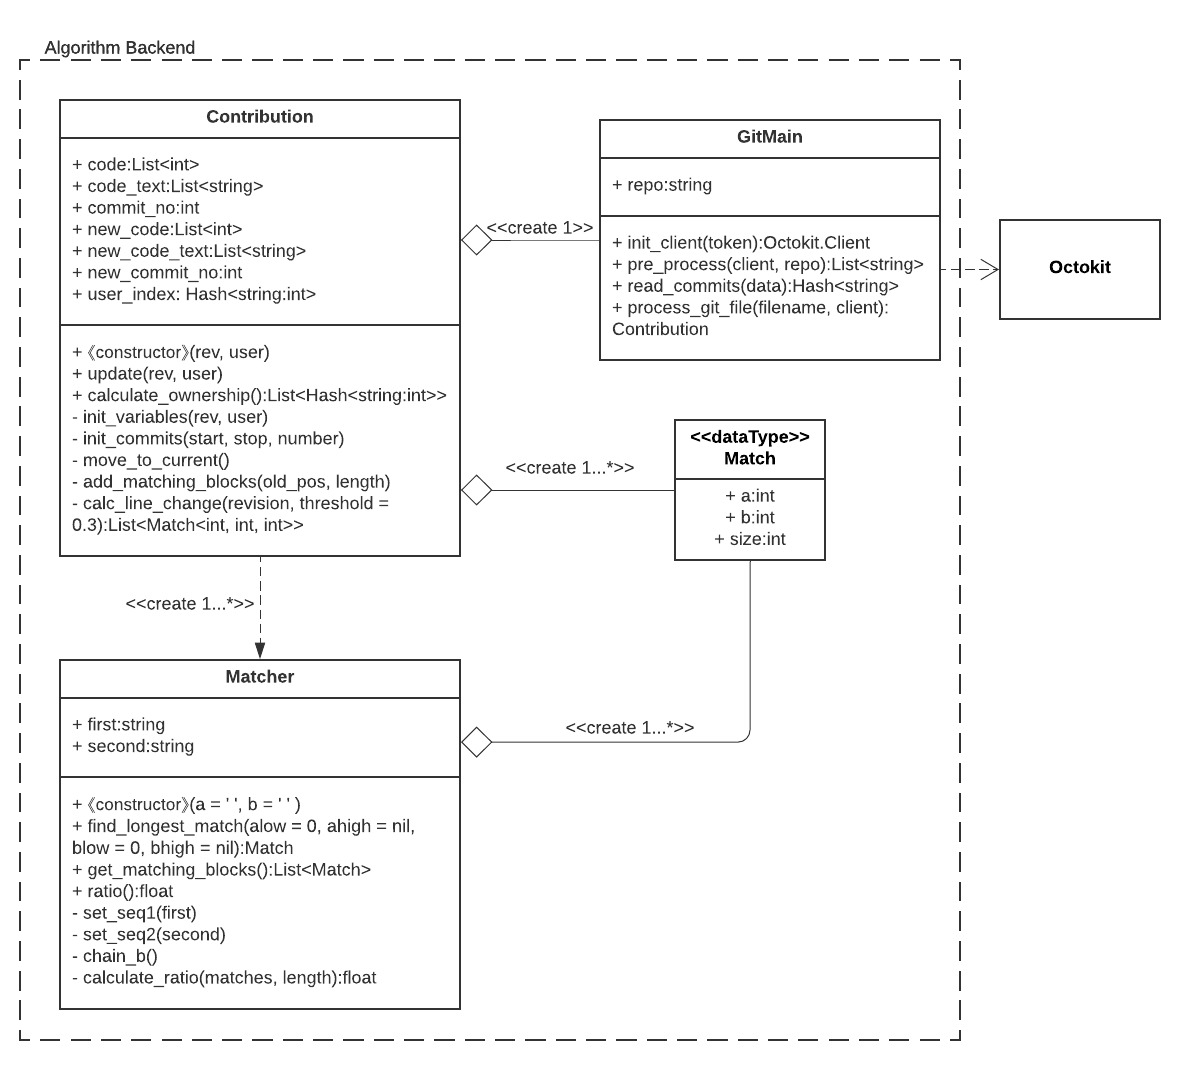
\includegraphics[scale=0.8]{images/UML class.jpeg}
    \caption{UML class diagram with a high-level overview of the application's back-end}
    \label{fig:7}
\end{figure}

The main components of the application's back-end can be seen above in Figure \ref{fig:7}. A brief description of each class can be seen below:
\begin{itemize}
    \item \textbf{Contribution}: The class containing the created algorithms that were discussed in Chapter 5 as Algorithm 1 and Algorithm 2.
    \item \textbf{Matcher}: The class that contains the Ruby implementation for the Gestalt Pattern Matching algorithm.
    \item \textbf{GitMain}: The class that implements the GitHub API calls for all the relevant repository required for the rest of the application.
\end{itemize}

\subsection{Front-end Infrastructure}

The front-end of the application is slightly more complex compared to the back-end as there are multiple views that utilise the Model-View-Controller (MVC) architecture as much as possible. The application starts off at a home page where the user is prompted to login using their GitHub account. If it is the user's first use of the application, they are then redirected to an external authorisation request from GitHub to allow the application to gain access to the user's basic profile details and their repositories. If the application is authorised by the user, the relevant controller retrieves the user's repository information and displays all of the user's repositories in a simple table. However, if the application is not authorised by the user, the user is redirected back to the home page. After the application is authorised, the user is then prompted to choose one of these repositories for analysis. When a repository is selected by the user, the application then queries the back-end of the application to get each file of the selected repository analysed by the \texttt{Contribution} class. Once the analysis is completed by the algorithms, the user is displayed with two different visualisations: a pie chart showing percentage contribution for each user, and a bar chart showing each user's persistence score. The view of this page also allows the user to change to some additional visualisations such as the ``Team View" and the ``File View".

When the ``Team View" button is clicked, the current page is reloaded to change the two visualisations from the original pie chart and bar chart to a more generalised version of these graphs. The currently logged in user would have their contributions compared to the rest of the team instead of each individual contributor. When the ``File View" button is clicked, a new page is displayed that lists all the files in the selected repository. The user can then click any of these files to get a new visualisation. This visualisation shows the selected file's contents at the most recent revision. The content of the file is then highlighted per character depending on the user that was attributed those changes by the algorithm. This gives the user a simple indication of how the algorithm works and allows the user to understand their contribution scores better.

In total, there are five different views for the application. The implementation of these views partially utilised the built-in CRUD (Create, Read, Update, Delete) routes for resources. For both the repositories list and the displaying of each repository's visualisations, the \text{Read} route mappings were utilised. For listing files in a repository and showing the file-based visualisation, the \texttt{Files} resource was set as a sub resource to the \texttt{Repos} to allow the file visualisation to be specific to each repository in the easiest implementation possible. Here, the \text{Read} route mappings were also utilised. The two \texttt{GET} routes utilised were \texttt{repos\#index} and \texttt{repos\#show} for both resources. Figure \ref{fig:8} shows the simple definition of the resources in lines 5-6.

\begin{figure}[h]
    \centering
    \begin{minted}[
    breaklines,
    frame=lines,
    framesep=2mm,
    baselinestretch=1.2,
    bgcolor=black,
    linenos]{ruby}
    Rails.application.routes.draw do
      root 'home#index'
      get 'home/index'
      get '/users/auth/github/callback', to: 'home#callback'
      resources :repos do
        resources :files
      end
    end
    \end{minted}
    \caption{Routes definitions in \texttt{routes.rb}}
    \label{fig:8}
\end{figure}

This meant that only 3 controllers were required for the entire application: \texttt{HomeController}, \texttt{ReposController} and \texttt{FilesController}. Below is the purpose of each controller:
\begin{enumerate}
    \item \texttt{HomeController}: Handle the callback route as defined in line 4 of Figure \ref{fig:8}. This callback route returns the authorisation code from GitHub and the controller carries out the exchange process discussed below in section 5.2.3 from step 4 to 5. Once the exchange is done, the user is redirected to the \texttt{repos\#index} view.
    \item \texttt{ReposController}: Handles both the \texttt{repos\#index} view and th \texttt{repos\#show} view. The \texttt{repos\#index} view displays a list of the user's repositories which is retrieved by the controller. The \texttt{repos\#show} view displays the visualisations specific to the selected repository. This controller is also responsible for converting the metrics produced for each file and amalgamating them to the data sets used for the ``Team" and ``Individual" visualisations. This involves accumulating the results for each file to a hash with a different key for each user.
    \item \texttt{FilesController}: Handles both the \texttt{files\#index} view and the \texttt{files\#show} view. It produces a list of the files in the selected repository for the \texttt{files\#index} view. For the \texttt{files\#show} view, the controller retrieves the selected file's attribution information from the \texttt{Contribution} algorithm, which is passed to the view to generate the highlighting of attribution for each user. 
\end{enumerate}

\subsection{GitHub integration}

The integration of GitHub accounts into the application was a complex process with many steps to get a user's authenticated information. Using the application as an authenticated user was essential for this application to have a higher API polling rate from 1000 requests per hour to 5000 requests per hour. One run-through of the application uses between 500 and 1000 API requests depending on the size of the repository so having this increased polling rate would allow the application to be run multiple times per hour. The process of authenticating a user is as follows:

\begin{enumerate}
    \item The user clicks on a Login button on the home page to start the authentication process. The link the user is sent to contains the client ID (which is created on the GitHub website) for the application and the requested scope of authorisation. 
    \item The button, when clicked, redirects the user to an external authorisation page on GitHub. This OAuth page requests for access to the user's personal user data and their public and private repositories for the application.
    \item If authorised, GitHub sends an authorisation code to the application. If unauthorised, the user is redirected to the home page.
    \item The authorisation code is then exchanged by the application for an access token using the application's client ID and client secret. This is done using one of the methods built into Octokit: \texttt{exchange\_code\_for\_token}. This method takes the authorisation code received from GitHub, the client ID and the client secret. It returns an access token which allows an \texttt{Octokit::Client} object to be created.
    \item The access is then passed from a temporary hash to a session variable. 
    \item The access token is passed into the constructor of the \texttt{Octokit::Client} class, which returns a \texttt{Client} object which can be used for all the API calls with the higher polling rate.
\end{enumerate}

\section{Testing and Verification}

As the application was being developed, branch testing was used extensively to ensure all branches were reached with the valid inputs needed for the branches to be reached. This type of testing was used mostly for verifying the algorithm and the many conditional statements used throughout the application. Branch testing was applied as each unit of the application was being developed, alongside verification tests to make sure these branches were both reached and returning the correct outputs. Once the application was at a working state and nearing completion, negative testing was employed to help identify any faults in the application. Erroneous data, such as empty files and new white space being added to files, were inputted to the algorithm using a benchmark data set (a GitHub repository with sets of erroneous files). \texttt{Begin-rescue} statements were used throughout the application to maintain the correct web flow for the application. An example of this is shown in Figure \ref{fig:9}, which occurs when the user does not authorise the application to their GitHub information.

\begin{figure}[h]
    \centering
    \begin{minted}[
    breaklines,
    frame=lines,
    framesep=2mm,
    baselinestretch=1.2,
    bgcolor=black,
    linenos]{ruby}
    def index
      ReposController.git = GitMain.new
      ReposController.client = ReposController.git.init_client(session[:access_token])
      begin
        @user = ReposController.client.user
        @profile_url = @user[:html_url]
        @user_name = @user[:name]
        @user_picture = @user[:avatar_url]
        @repos = ReposController.client.repos(access_token: session[:access_token])
      rescue Octokit::Unauthorized
        redirect_to '/'
      end
    end
    \end{minted}
    \caption{Error handling in \texttt{ReposController}}
    \label{fig:9}
\end{figure}

This example of error handling tries to initialise a \texttt{Octokit::Client} object in line 3 using the access token currently stored for this session. As previously discussed in Section 5.2.3, the access token is retrieved through an exchange process. If the user does not authorise the application, the exchange process still occurs but the process returns an unauthorised access token. This results a \texttt{Octokit::Unauthorized} exception to be thrown when a \texttt{Octokit::Client} object is created and attempted to be queried. When this occurs, the user is redirected back to the home page so they can authorise the application.

Unit testing was also heavily utilised for both the front-end and the back-end of the application in completing both branch and negative testing. An example of a unit test implemented in the application is \texttt{HomeControllerTest} as shown in Figure \ref{fig:10}. This test is a simple verification test to check the home page is reachable with a successful HTTP response code (200 - 299). 

\begin{figure}[h]
    \centering
    \begin{minted}[
    breaklines,
    frame=lines,
    framesep=2mm,
    baselinestretch=1.2,
    bgcolor=black,
    linenos]{ruby}
    require 'test_helper'

    class HomeControllerTest < ActionDispatch::IntegrationTest
      test "should get index" do
        get home_index_url
        assert_response :success
      end
    end
    \end{minted}
    \caption{Unit test in \texttt{HomeControllerTest}}
    \label{fig:10}
\end{figure}

\section{Maintainability}

Maintainability is a key feature to be considered when evaluating a software project. When developing the application, maintainability was one of the most important factors considered when making changes to the application. During the design of the application, it was important to keep the cohesion between modules in the application to be as high as possible. Coupling was also another characteristic that was considered at the design stage to keep this as loose as possible. Figure \ref{fig:7} clearly shows some of these considerations. It's clear to see from the class diagram that the application has minimal dependencies between each class/module (from the limited number of lines between each class). There is also a limited number of external dependencies since the pattern matching algorithm was coded from scratch and the GitHub integration only required one library to be installed, Octokit. This promotes loose coupling between modules and makes sure no module is over reliant to any other module. For example, no module relies on the overarching \texttt{Contribution} class. Additionally, attribute accessors (``getters") and mutators (``setters") were used to prevent implicit coupling and keep information regarding a class encapsulated. Reducing as many instances of coupling maximises an application's maintainability since each module can be reused and easily be tested independently. New modules can also be easily added to the application as there is no current dependencies within modules that need to be mimicked in new modules.

Figure \ref{fig:7} also demonstrates high cohesion within each module. Exemplar to this, each controller is concerned only with the views they are controlling. This is facilitated by the built in framework from Ruby on Rails to promote the Model View Controller design pattern. By default, the design pattern makes sure the views are separate from the logic of the application. This makes sure that the display and the data are able to change without affecting the other. One place the high cohesion is adamant is in the \texttt{FilesController}. Since the files retrieved for the \texttt{files/index} page depends on the selected repository, one could create an instance of the \texttt{ReposController} to have access to all the properties necessary for the view to be generated. However, this can give the class access to attributes that are not needed by it. Instead, \texttt{ReposController} defines attribute accessors that are needed by the \texttt{FilesController} and they are simply called by the class (as seen in Figure \ref{fig:11}). This helps eliminate any DRY (Don't Repeat Yourself) code for retrieving filenames.

\begin{figure}[h]
    \centering
    \begin{minted}[
    breaklines,
    frame=lines,
    framesep=2mm,
    baselinestretch=1.2,
    bgcolor=black,
    linenos]{ruby}
    def index
      @repo_name = ReposController.repo_name
      @files = ReposController.files
    end
    \end{minted}
    \caption{Logic for the \texttt{files/index} view in \texttt{FilesController}}
    \label{fig:11}
\end{figure}

Following coding style is another way to keep an application maintainable. If a large codebase has a high quality but follows no existing styling standards, the software becomes a difficult problem for maintaining in the future. For the application, RubyMine's built-in integration of The Ruby Style Guide \citep{batsov_2021} (using RuboCop) was integral in following these styling guidelines. These guidelines are very similar to and inspired by Python's PEP 8 style guide. One of the most important parts of the style guide is to use descriptive identifiers for all units of the application such as classes, methods and variables. An example of this in the application is \texttt{calculate\_ownership()} method in the \texttt{Contribution} class which calculates each user's separate contributions.
%\chapter{Professional Issues}
This section explores the various professional issues and the legislation involved with the project. The issues considered include any legal, social, ethical or professional issues. Discussed will also be adherence and any issues with regards to the British Computing Society's Code of Conduct and Code of Good Practice \citep{bcsconduct}.

\section{Issues}
The developed system uses a collection of open source libraries such as Chartkick, Octokit and a number of RubyGems that are conventional for Ruby on Rails projects. This includes Turbolinks, a framework used to improve single-page performance when loading pages via buttons and hyperlinks, and \texttt{sass-rails}, the official Ruby-on-Rails integration of the stylesheet language Sass (Syntactically Awesome Style Sheets). The difference between work created as part of this project and work of others has been explained succinctly throughout this report. Most of the libraries used in this project have licenses permitting use within commercial applications. However, if the application was sold commercially or started making money, a lot of the library choices may require rethinking.

The created application has use of users' information through an API, which has more issues that need to be handled. Firstly, only information required by the application is retrieved from GitHub and it is only used during a single session, after which the information is discarded. No information is stored and all instances of the application are independent of one another. Secondly, the communication between the application and the GitHub API is encrypted using HTTP/SSL. This means if an attacker tried to intercept a user's information, the data the attacker is unreadable without a private key.  

\section{Code of Conduct}
When designing and implementing of the application, a significant consideration was made to make sure that the process of developing the application followed the British Computer Society's (BCS) Code of Conduct \& Code of Good Practice. The developed application does not provide any functionality that could be utilised to cause misuse. 
%\chapter{Evaluation}
This chapter aims to examine and explore the application when being compared with existing algorithms. This will be done using benchmark tests between the applications and its competitors. 

\section{Comparisons}

For this project, three different scales of repositories were utilised for testing and comparison. This provided both validation for the underlying algorithm and a comparison of the algorithm's performance in different scenarios. The four repositories used were: Minetest \citep{ahola_2021}, a C++ ``open-source voxel game engine" similar to Minecraft; HospitalHeroes, a mobile application created as part of the Software Engineering Major Project written in Java; dplyr, a grammar created for data manipulation for the R programming language written in R. Minetest was chosen for its sheer size and its high level of crowdsourcing; as of April 2021, the repository had 9,337 commits made by 523 contributors. This repository is a great test for the application as it has around 1000 files with a large range of programming languages for many different purposes such as Python, C++, Bash, Lua and HTML. HospitalHeroes was chosen since it was created in the same environment that the application will be integrated into. It is a student group software engineering project which is the target dataset for this application. This project is much smaller than the aforementioned Minetest repository; the repository has 445 commits from only 7 contributors. Lastly, dplyr was chosen to represent a repository that is between the other two repositories; the repository has 7,109 commits from 244 contributors. A collection of binary-based files (namely jar, png, bmp, dll, jpg, jpeg, exe, ttf, ico, icns, svg, ogg, mp3, wav and bat files) were excluded from this project as the algorithm analyses text-based files and not binary files. 

Different repository managers usually differ in the way they distinguish who makes and how changes made to files. For instance, Apache Subversion does not differentiate a user that commits the changes (the committer) and the user that actually made the changes (the author). On the contary, \texttt{git} and its many repository managers (e.g. GitHub, Gitlab, BitBucket) actually differentiates the author from the committer, which allows the application to accurately contribute changes to the author. 

\subsection{Correlation-based Comparison}

For the following measures, the commits were retrieved for each repository per file. For users that contributed to more than one file, their scores were combined for all the different measures. The measures that will be compared are the numerous measure discussed previously in Section 2.2 alongside this project's proposed contribution algorithm. The Kendall rank correlation coefficient (often referred to as Kendall's $\tau$ rank correlation) was used to compare whether the various ranking methods agree with the result received. Since tau values are bounded between 0 and 1, it is easy to evaluate the agreements between each measure. These results can be seen below in Tables \ref{table:1}, \ref{table:2}, and \ref{table:3}. The proposed algorithm is referred to as Algo in these tables.

\begin{table}[ht]
    \centering
    \begin{tabular}{l l l l l l l l}
         \hline
         & Commits & Touch & LOC & gitauthor & Chars & Algo & T \\
         \hline
         Commits & 1 & & & & & & \\
         Touch & 0.563 & 1 & & & & & \\
         LOC & 0.488 & 0.669 & 1 & & & & \\
         gitauthor & 0.486 & 0.567 & 0.781 & 1 & & & \\
         Chars & 0.505 & 0.533 & 0.720 & 0.825 & 1 & & \\
         Algo & 0.586 & 0.679 & 0.576 & 0.623 & 0.684 & 1 & \\
         T & 0.349 & 0.443 & 0.356 & 0.365 & 0.346 & 0.381 & 1 \\
         \hline
    \end{tabular}
    \caption{Kendall tau for Minetest}
    \label{table:1}
\end{table}

\begin{table}[ht]
    \centering
    \begin{tabular}{l l l l l l l l}
         \hline
         & Commits & Touch & LOC & gitauthor & Chars &  Algo & T \\
         \hline
         Commits & 1 & & & & & & \\
         Touch & 0.322 & 1 & & & & & \\
         LOC & 0.327 & 0.854 & 1 & & & & \\
         gitauthor & 0.319 & 0.723 & 0.847 & 1 & & & \\
         Chars & 0.242 & 0.648 & 0.724 & 0.848 & 1 & & \\
         Algo & 0.284 & 0.699 & 0.683 & 0.768 & 0.843 & 1 & \\
         T & -0.202 & 0.370 & 0.300 & 0.310 & 0.392 & 0.379 & 1 \\
         \hline
    \end{tabular}
    \caption{Kendall tau for HospitalHeroes}
    \label{table:2}
\end{table}

\begin{table}[ht]
    \centering
    \begin{tabular}{l l l l l l l l}
         \hline
         & Commits & Touch & LOC & gitauthor & Chars &  Algo & T \\
         \hline
         Commits & 1 & & & & & & \\
         Touch & 0.285 & 1 & & & & & \\
         LOC & 0.283 & 0.878 & 1 & & & & \\
         gitauthor & 0.301 & 0.728 & 0.782 & 1 & & & \\
         Chars & 0.306 & 0.644 & 0.694 & 0.814 & 1 & & \\
         Algo & 0.316 & 0.674 & 0.667 & 0.767 & 0.899 & 1 & \\
         T & 0.166 & 0.422 & 0.387 & 0.369 & 0.356 & 0.357 & 1 \\
         \hline
    \end{tabular}
    \caption{Kendall tau for dplyr}
    \label{table:3}
\end{table}

The proposed algorithm can clearly be seen to agree with the rest of the measures. This is a great indicator showing the results produced by the algorithm are not inordinately different from those produced by the other measures. The way the Kendall coefficient works is a positive coefficient means that as a score from one ranking system rises, the other ranking system also increases proportionally. On the other hand, negative coefficients show that users are ranked in reverse when compared between two measures. Any results near zero show that the results have no correlation, showing a ranking system produces poor results. Luckily, the algorithm in this project does not produce these kind of results. Instead, the algorithm produces results that are not too dissimilar to those from other ranking measures. The largest dissimilarity between any measures can be seen from the \textit{T} measure, which is expected since \textit{T} is the only measure that looks at time as opposed to textual elements of the code. The algorithm is most correlated with \textit{gitauthor} and \textit{Chars} due to the fact the algorithm is partly a character based measure. The only negative coefficient can be seen between the \textit{Commits} and \textit{T} measures in the HospitalHeroes repository. This shows that \textit{Commits} is limited in its measurement of contribution since all other methods of ranking have a positive coefficient with the \textit{T} measure. For instance, a succession of commits in a short time span (e.g. code churn) for a user is not the same as large work sessions, which is what the \textit{T} measure represents.

However, it is clear that the algorithm is not in complete accordance with any existing ranking measures. This is as expected since the algorithm looks to include extra factors when regarding the final rankings and engulfs a lot of these different measures together.

\section{Performance}

Using the algorithm for analysing a repository is a resource intensive task. When trying to calculate a time complexity, there is a lot of different levels of abstraction that can be analysed and a lot of external factors to consider involving the repository and how the contributors work. For example, a repository with a small number of commits that all have large amounts of line changes associated with them will allow the algorithm to run much faster than a repository with a large number of smaller sized commits. 

From a high level overview, the application's runtime is dependant on the number of commits $N$ that each file is associated with $f(O(N))$. However, iterating over previous commits is not necessary every time a new commit is made to the repository. The use of the \textit{Y} variable can be expanded to store the variable's last state. When a new commit is made to the repository, the stored $Y$ can be retrieved and reprocessed with the new commit. This will result in a smaller time complexity of $O(1)$ while losing space for storing a version of $Y$ for each file in the repository.  

At a lower level of abstraction, between each two revisions ($r_i$ and $r_{i-1}$) that contain the lines $l_i$ and $l_{i-1}$, a double for loop is instantiated. The best case scenario for this loop is $O(l_i)$ when $l_i \geq l_{i-1}$ or $O(l_{i-1})$ if $l_i < l_{i-1}$. However, the worst case means that the resulting time complexity is $O(l_i * l_{i-1})$, meaning each line of $r_i$ is compared at least once with each line of $r_{i-1}$. When new lines are detected, the Gestalt algorithm is run on the entire text for $r_i$ and $r_{i-1}$. This results in a quadratic worst case of $O(n * m)$ where $n$ and $m$ are the number of characters in each revision. Practically, the greatest causes of time overhead for a calculation to finish are the number of commits in a repository and the average number of lines in each file of the repository.
%\chapter{Conclusion and Future Work}

The project's conclusions should list the key things that have been learnt as a consequence of engaging in your project work. For example, ``The use of overloading in C++ provides a very elegant mechanism for transparent parallelisation of sequential programs'', or ``The overheads of linear-time n-body algorithms makes them computationally less efficient than $O(n \log n)$ algorithms for systems with less than 100000 particles''. Avoid tedious personal reflections like ``I learned a lot about C++ programming...'', or ``Simulating colliding galaxies can be real fun...''. It is common to finish the report by listing ways in which the project can be taken further. This might, for example, be a plan for turning a piece of software or hardware into a marketable product, or a set of ideas for possibly turning your project into an MPhil or PhD.

%%%%%%%%%%%%%%%%%%%%%%%%%%%%%%%%%
% References
%%%%%%%%%%%%%%%%%%%%%%%%%%%%%%%%%
\addcontentsline{toc}{chapter}{Bibliography}
\bibliographystyle{agsm}
\bibliography{bibliography}

%%%%%%%%%%%%%%%%%%%%%%%%%%%%%%%%%
% Appendices
%%%%%%%%%%%%%%%%%%%%%%%%%%%%%%%%%
%\appendix
\chapter{Appendix}
\section{Appendix 1: Proof of Claim 1}
\begin{proof}
Let $\left \lfloor x \rceil \right \in \mathbb{Z}^+$ be the closest integer to \textit{x}. The following holds: 
\begin{align*}
x - \frac{1}{2} \leq \left \lfloor x \rceil \right \textless x + \frac{1}{2}
\end{align*}

For $x = n * threshold$ where $n > 0$ and $threshold \in \mathbb{R} \mid 0 < threshold \leq 1$:
\begin{align*}
n * threshold - \frac{1}{2} \leq \left \lfloor n * threshold \rceil \right \textless n * threshold + \frac{1}{2}\\
\longrightarrow \frac{n * threshold - \frac{1}{2}}{n} \leq \frac{\left \lfloor n * threshold \rceil \right}{n} < \frac{n * threshold + \frac{1}{2}}{n}\\
\longrightarrow \frac{n * threshold}{n} - \frac{\frac{1}{2}}{n} \leq \frac{\left \lfloor n * threshold \rceil \right}{n} < \frac{n * threshold}{n} + \frac{\frac{1}{2}}{n} \\ 
\longrightarrow threshold - \frac{1}{2n} \leq \frac{\left \lfloor n * threshold \rceil \right}{n} < threshold + \frac{1}{2n} \\
\longrightarrow mt - mt - \frac{1}{2n} \leq \frac{\left \lfloor n * threshold \rceil \right}{n} - mt < mt - mt + \frac{1}{2n}
\end{align*}

Since the middle section of the equality can be interpreted as the error when applying a percentage over a discrete data set, we can call this as \textit{d} \citep{stephen_post_2017}. So:
\begin{align*}
-\frac{1}{2n} \leq d < \frac{1}{2n}\\
\longrightarrow \abs{d} \leq \frac{1}{2n}
\end{align*}
Therefore the maximum of \textit{d} is $\abs{d_{max}} = \frac{1}{2n}$.
\end{proof}


%\chapter{User Guide}
\section{Instructions}
You must provide an adequate user guide for your software. The guide should provide easily understood instructions on how to use your software. A particularly useful approach is to treat the user guide as a walk-through of a typical session, or set of sessions, which collectively display all of the features of your package. Technical details of how the package works are rarely required. Keep the guide concise and simple. The extensive use of diagrams, illustrating the package in action, can often be particularly helpful. The user guide is sometimes included as a chapter in the main body of the report, but is often better included in an appendix to the main report.

%\chapter{Source Code}

\thispagestyle{empty}
\begin{center}
    \textbf{Originality Avowal}\\*
    \begin{flushleft}
        I verify that I am the sole author of the programs contained in this folder, except where explicitly stated to the contrary. \\
    \end{flushleft}
    \begin{flushright}
        \normalsize{Fahim Mohammed}\\*
        \normalsize{April 7, 2021}\\*
    \end{flushright}
\end{center}

\section{Table of Contents}

\begin{center}
\begin{tabular}{ | m{15em} | m{18em}| m{4em} | } 
\hline
\textbf{Filename} & \textbf{Description} & \textbf{Page \#} \\ \hline

Gemfile & File containing all the Ruby dependencies for the project & 1 \\ \hline
.gitignore & All directories and extensions ignored for version control & 2 \\ \hline
gitmain.rb & GitHub API integration for retrieving relevant repository info & 4-5  \\\hline
matcher.rb & Implementation of the Gestalt pattern matching algorithm & 6-8 \\ \hline
contribution.rb & The main algorithm created as a part of this project & 9-12 \\ \hline
home/index.html.erb & View for homepage of the application & 13 \\ \hline
files/show.html.erb & View for displaying per file visualisation & 14 \\ \hline
files/index.html.erb & View displaying all the files in a repository & 15 \\ \hline
repos/show.html.erb & View displaying visualisations for a given repository & 16  \\ \hline
repos/index.html.erb & View listing all the private and public repositories of a user & 17 \\ \hline
layouts/files.html.erb & Custom layout for the per file visualisation & 18 \\ \hline
layouts/application.html.erb & Default layout file for all other views & 19 \\ \hline
home.scss & Stylesheet for homepage & 20 \\ \hline
files.scss & Stylesheet for file-based views & 21 \\ \hline
repos.scss & Stylesheet for repository list & 22 \\ \hline
application.scss & Stylesheet for entire application & 23 \\ \hline
auth-buttons.css & Stylesheet for button on homepage & 24-26 \\ \hline
helpers/application\_helper.rb & Helper that is used to start GitHub authorisation & 27 \\ \hline
controllers/home\_controller.rb & Controller for the homepage & 28 \\ \hline
controllers/files\_controller.rb & Controller for all the file-based views & 29 \\ \hline
\end{tabular}

\begin{tabular}{ | m{16em} | m{18em}| m{4em} | } 
\hline
\textbf{Filename} & \textbf{Description} & \textbf{Page \#} \\ \hline
controllers/repos\_controller.rb & Controller for the repo list and the repo visualisation & 30-31 \\ \hline
controllers/application\_controller.rb & Abstract controller that is inherited by other controllers & 32 \\ \hline
config/routes.rb & Routes page that controls the URLs of the application & 33 \\ \hline  
config/application.rb & The main application file where all other Ruby files are automatically loaded & 34 \\ \hline
config/application.yml & Environmental variables used for GitHub integration & 35 \\ \hline
\end{tabular}
\end{center}


\end{document}
